% !TeX root = ../main.tex

\chapter{系统需求分析及架构设计}
本章节系统全面介绍了视频表决会议系统的需求分析及架构设计工作。本章节从系统业务出发,分析了视频表决会议系统的需求,根据需求进行了针对性的架构设计,并介绍了与原会议系统的区别之处。

\section{需求分析}

会议系统根据功能性质划分,分为两个大的模块,一是会议管理模块,另一个是会议系统主模块。运营平台会议管理模块负责会议的创建、修改及数据导入等会议管理功能。会议系统主模块负责视频直播、投票表决、实时查看数据、实时聊天等会议核心功能。

\subsection{会议管理模块}

会议系统管理模块负责会议管理相关的功能,会议的管理模块由运营人员在运营平台进行操作,运营人员具有的功能权限有创建/修改会议、导入表决数据、导入其他参会人员信息、获取密码反馈、激活会议、发送短信通知及获取推流地址。会议系统管理模块的具体功能需求如图~\ref{fig:meetingManagement} 所示。

\begin{figure}[!htp]
  \centering
  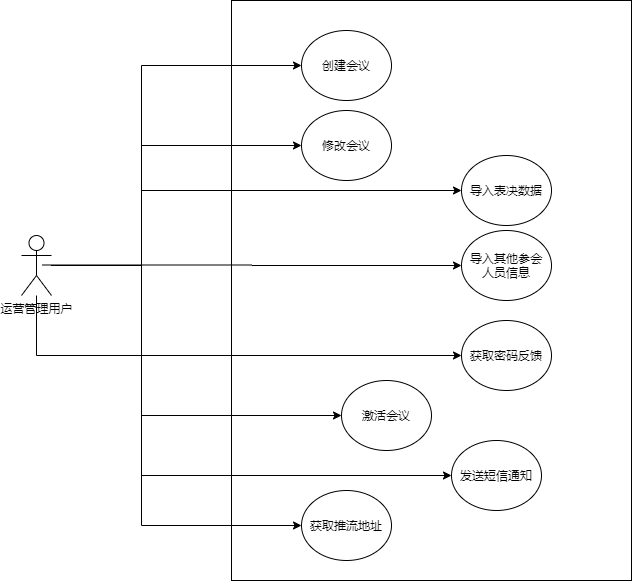
\includegraphics[height=8cm]{meetingManagement.png}
  \bicaption[管理模块]
    {会议系统管理模块需求用例图}
    {Meeting management module requirements use case diagram}
 \label{fig:meetingManagement}
\end{figure}

\subsubsection{创建和修改会议}
原系统会议模块创建和修改会议分为三步,填写会议基本信息、填写议题相关信息、导入议题表决信息。导入议题表决信息显然和创建会议属于不同功能,将导入信息作为创建会议的一环并不合理,因此将导入议题表决信息功能单独拆出。另外将创建会议拆分成两步并没有实际意义,反而增加了创建会议时出现错误的概率,因此将填写会议基本信息、填写议题相关信息合并为一步。

运营管理人员在运营平台创建和修改会议。创建和修改会议需要填写会议的基本信息(会议名称和会议召开日期为必填项)、会议的议程信息(包括需表决和无需表决议程)、议程的表决组信息,由于向 OSS 文件系统存储会议文件和议程文件时,需要会议号作为索引,因此在创建会议前需要提前向后端请求获取预约会议号。

\subsubsection{导入表决数据和其他参会人员信息}
表决数据包括表决信息(表决所在表决组、表决金额等)和表决信息对应的债权人信息。原系统会议模块导入表决数据是创建会议的第三步,表决数据仅可导入原债权申报系统中已存在的数据,若仅使用会议功能,表决数据的导入和原债权申报系统数据强绑定的设计就显得极为不合理。因此将导入表决数据和原债权申报系统数据解除绑定,改为使用 Excel 文件上传导入表决数据。点击下载 Excel 模板,填写完表决数据完整信息后,点击导入表决数据上传填好的 Excel 文件。此时,可能存在债权人未在会议平台注册的情况,表决数据若对应已存在债权人,则将表决数据划分给已存在债权人。表决数据若对应不存在债权人,则先创建对应债权人,再将表决数据划给创建的债权人。

会议除相关管理人和债权人外,还存在其他参会人员(仅可观看会议)。其他参会人员不可自行注册,仅可通过运营人员在运营平台通过上传 Excel 文件导入,目的是为了防止会议无关人员参与会议。

\subsubsection{发送短信通知}
与原系统会议模块相比,增加了短信通知功能。运营平台管理员可以向所有会议相关人员发送短信通知。选定模板和发送范围后,可以向指定范围发送会议相关信息。

\subsection{会议系统主模块}

原系统会议模块用户分为两类。一是管理人用户,二是债权人用户。若存在仅可观看会议的其他类型参会人员,需注册为债权人用户,不赋予表决数据,即可满足只能观看的需求。这种做法不符合规范,因此新增游客用户类型,仅提供观看会议的权限。

会议系统主模块负责会议的核心功能。视频表决会议系统的用户分为三类。一是管理人用户,二是债权人用户,三是游客用户(即其他参会人员)。管理人用户具有开启表决、结束表决、查看表决详情、查看参会详情、设定结束日期、查看会议详情、查看会议列表、观看视频直播、实时聊天的功能。债权人用户具有签到、补签、投票表决、实时聊天、查看会议列表、查看会议详情、观看视频直播的功能。游客用户具有查看会议列表、查看会议详情、观看视频直播的功能。会议系统主模块的具体功能需求如图~\ref{fig:meetingMain} 所示。

会议系统主模块功能根据是否有实时性要求又分为实时模块和非实时模块。实时模块包括实时聊天功能和投票表决功能。

\begin{figure}[!htp]
  \centering
  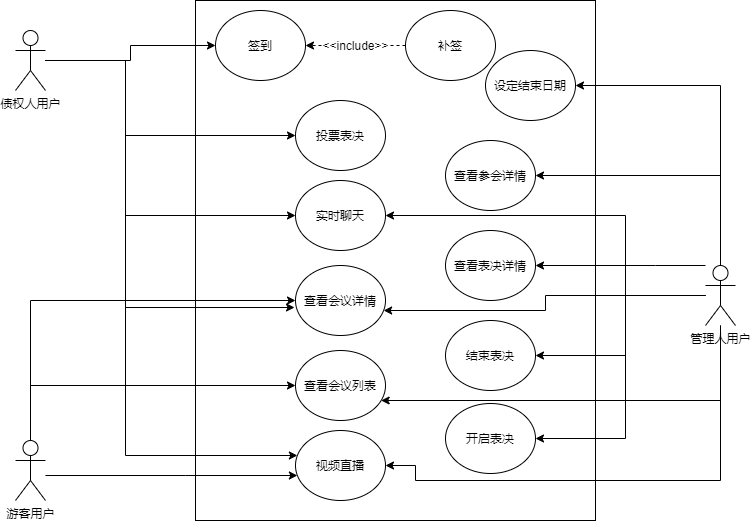
\includegraphics[width=10cm]{meetingMain.png}
  \bicaption[主模块]
    {会议系统主模块需求用例图}
    {Meeting main module requirements use case diagram}
 \label{fig:meetingMain}
\end{figure}

\subsubsection{开启和结束表决}
原系统会议模块的表决开启和结束由创建会议时设定的开启日期和结束日期决定,由于实际需求中,会议的表决开启和结束有时需要管理人进行控制,因此管理人用户增加了开启和结束表决的功能。

\subsubsection{查看参会详情和表决详情}
原系统会议模块仅有参看表决详情功能。在实际的会议中,管理人有时需要向法院报告会议参会情况,因此管理人用户增加了查看表决详情的功能。

\subsubsection{签到和补签}
原系统会议模块中,债权人参加会议功能在任何时间都可以使用,即时会议已经结束,债权人仍可点击参会,这与常理不符。现在改为债权人在会议开始到会议结束之间第一次进入会议时,会主动弹出签到框,提醒债权人签到参会,并提供补签功能,签到成功后才可进行投票表决。

\section{架构设计}
在破产领域中,债权人会议和表决的意义十分重大,决定着一个破产项目的走向。在一次实际的债权人会议中,债权人的数量级平均为千人级别,有些会议的债权人数量甚至可以达到上万人。债权人会议的一项重要工作是进行表决。在实际的会议中,表决可能在较短的时间内进行,因此会导致在短时间内出现大量请求。当同时有多个会议进行时,短时间激增的请求会给服务器带来极大的压力,因此需要针对性的设计架构应对此问题。

\subsection{现有架构及问题}

\subsubsection{现有架构}
\begin{figure}[!htp]
  \centering
  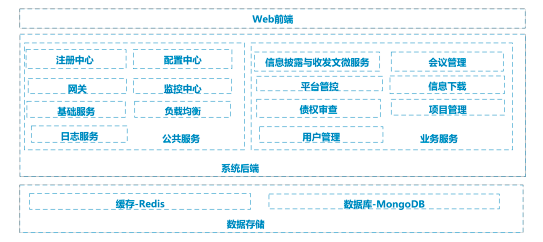
\includegraphics[width=12cm]{oldMeeting_1.png}
  \bicaption[原微服务]
    {原系统微服务架构图\cite{Wang2021}}
    {Original system microservice architecture diagram\cite{Wang2021}}
 \label{fig:oldMeeting_1}
\end{figure}

原系统采用微服务架构的原因一是原系统已具有比较完整
的服务治理管理体系,采用微服务架构将节省部署运维和降低系统升级的工作难度。这样
就能充分复用原系统的实现,减少开发系统,升级系统的成本。二是可以满足系统可
扩展性的要求。当需要对系统持续升级与优化时,可以直接设计其他微服务加入到微
服务治理体系中以满足用户不断扩展的需求。具体架构如图~\ref{fig:oldMeeting_1}\cite{Wang2021} 所示。根据微服务架构设计的高内聚低耦合的原则,原系统将会议管理整体划分为一个微服务,所有会议相关的功能全部集中放在会议管理微服务中。

在原系统的设计中,当用户数上升时,可以为各个微服
务起多个实例同时服务来满足用户并发数,可以在不改变软件架构的基础上通
过增加硬件资源来提高服务质量。

原系统是在 k8s 集群上进行部署的,系统采用图~\ref{fig:oldMeeting_2}\cite{Wang2021}
的物理架构。系统用户可以直接通过浏览器访问系统。而用户的请求都将到达 K8s 集群中
的 Mater Node,由 Master Node 结点进行处理。Mater Node 结点是整个集群的管理结点,该
结点会根据请求的特性命令 Work Node 结点进行作业工作。另外,一个服务往往运行成多个实例以增加系统的容错性。

\begin{figure}[!htp]
  \centering
  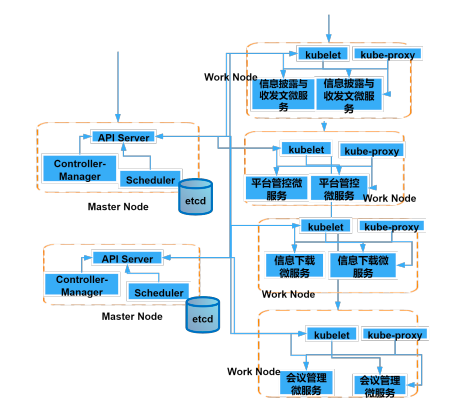
\includegraphics[height=6cm]{oldMeeting_2.png}
  \bicaption[原物理架构]
    {原系统物理架构图\cite{Wang2021}}
    {Physical architecture diagram of the original system\cite{Wang2021}}
 \label{fig:oldMeeting_2}
\end{figure}

\nocite{Wang2021}
\subsubsection{存在问题}

在网络债权人会议中,保证实时性非常重要。在原系统的实现中,会议管理微服务实现为 SpringBoot 后端,在会议管理微服务中通过 WebScoket 实现实时聊天,通过轮询实现管理人查询数据的实时更新。

首先,假设系统需要能同时处理 1 万场会议,每个会议债权人数量为 1万人,仅仅实时聊天的长链接数量就达到了1亿级别。SpringBoot 项目的默认启动容器是 Tomcat,而 Tomcat 默认支持的连接数量为 1 万,这个数量级远远低于要求。如果将 Websocket 实现在 SpringBoot 项目中,需要调大 Tomcat 的连接数量或者更换启动容器,即使更换启动容器将连接数量扩大至百万级,按照原系统设计为会议管理微服务起多个实例同时服务来满足并发数需要启动接近1百个实例,这仅仅是为了满足保持实时聊天的长连接数量。

其次,通过轮询方式实现管理人端查看数据的实时更新,会给服务器带来较大的压力,且比较浪费资源,债权人侧投票表决和管理人侧数据实时刷新也应当通过 WebScoket 实现。

我们发现在会议系统中,需要通过 WebScoket 实现的功能和其余功能是独立的,并且在现有设计下为了保证 WebScoket 的长连接数量会给服务器带极大压力和资源浪费,因此考虑将 WebSocket 相关功能拆出实现为独立的微服务。

\subsection{架构设计}
将原本的会议管理微服务拆分为会议管理微服务(除去实时功能)、实时表决微服务和实时聊天微服务。新的会议管理微服务仅包含基础功能(创建会议等),与原本实现差别不大。会议开始前和会议结束后的表决数据查询通过会议管理微服务,而在会议进行中时,表决数据查询通过实时微服务进行,后面主要介绍实时微服务架构设计。

针对系统的某个实时微服务,如表决服务、聊天服务,所有用户均使用同一套服务架构。
该服务架构一定包括无状态的 WebSocket 实例(后文简称 “实例”),以及独立的有状态 Redis 服务。Redis 服务是实例的状态中心,存储实例的所有状态数据。
采用分布式集群方案,服务架构如图~\ref{fig:cluster}。

\begin{figure}[!htp]
  \centering
  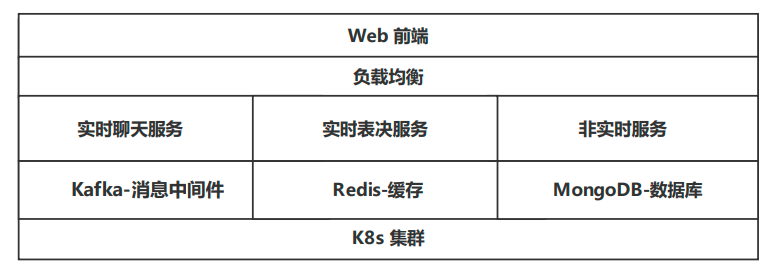
\includegraphics[width=12cm]{cluster.png}
  \bicaption[实时微服务架构]
    {实时微服务架构图}
    {Real-time microservices architecture diagram}
 \label{fig:cluster}
\end{figure}

\subsubsection{数据分类}

\begin{figure}[!htp]
  \centering
  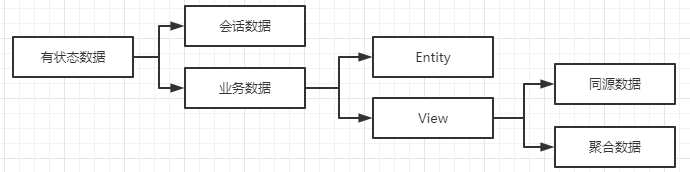
\includegraphics[width=12cm]{dataClassification.png}
  \bicaption[数据分类]
    {数据类型分类示意图}
    {Schematic diagram of data type classification}
 \label{fig:dataClassification}
\end{figure}

如图~\ref{fig:dataClassification},影响实例外在表现的所有副作用数据统称为有状态数据。
有状态数据分为两类,一类是会话数据,一类是业务数据。其中会话数据及业务数据中的Entity数据存于 Redis 中,其余数据均只存于实例内存中。

会话数据为连接的元信息,例如用户 Id ,聊天室 Id , jwt 验证信息等等。
在用户刚刚与实例建立连接时,实例将初始化好用户的会话数据并将其暂存于 Redis 中。
会话数据为每个用户对每个服务的独有数据,包含用户、连接、权限三者的元信息。
用户下线后,会话数据将会被清除。
同用户异地登录,所建立的会话会将原有会话顶替下线(实时服务一账号只可一人用)。

业务数据为影响用户前端展示的数据。例如:某债权人的表决情况,某会议的总签到人数等。
业务数据又分为 View 和 Entity 两种数据。

Entity 为 Mongo 中存储的真实数据,实例会将其暂存于 Redis 中。View 数据是抽象概念,指将对某类用户前端视图展现的全量信息。例如:管理人可见的表决统计总表数据,或者整个聊天室的所有聊天内容和封禁状态。View 并非 Mongo 内的实体数据,往往是多个 Entity 的聚合数据,或者是全体 Entity 的子集。View 数据内部包含同源数据与聚合数据两类。

同源数据是全体 Entity 的子集,内存中为至 Entity 的索引。以保证完全与 Entity 数据保持一致。比如某债权人对某表决是否投票,投了同意还是反对。

聚合数据是由 Entity 聚合而出的数据,会随着某些 Entity 的改变而改变。比如某个会议下某议题的总同意金额。

同源数据和聚合数据采用不同结构存储。它们的区分是调和 “性能” 与 “数据一致性” 矛盾的基石,下节数据存储将会介绍。

\subsubsection{数据存储}

\begin{figure}[!htp]
  \centering
  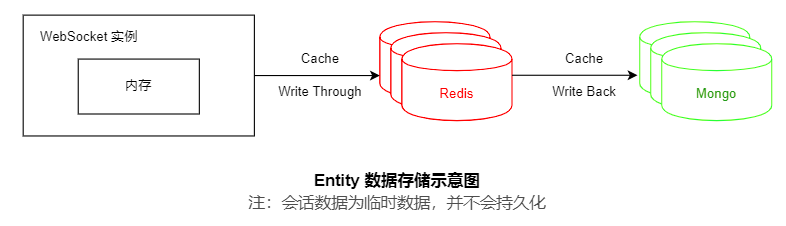
\includegraphics[width=12cm]{dataSave.png}
  \bicaption[Entity存储示意]
    {Entity存储示意图}
    {Entity Storage Diagram}
 \label{fig:dataSave}
\end{figure}

不同类的业务数据存储形式不同。Entity 数据最终会持久化至 Mongo。Entity 被分散到三处。实例内存是 Redis 的 Cache,而 Redis 事实上是 Mongo 的 Cache。

实例必须无状态,其状态必须可从 Redis 恢复。因此实例内存至 Redis 为 Write Through 策略。实际测试得知 Mongo 仅支持 100+qps ,为性能瓶颈,在实验一节中会详细描述。因此 Redis 至 Mongo 为 Write Back 策略。如图~\ref{fig:dataSave}所示。

View 数据只保存在实例内存中。View 内部存储的同源数据事实上只是到某些 Entity 的映射(id、指针等)。View 内部存储的聚合数据是对应的聚合后的计算值。由于 View 内部存储的事实上只是 Entity 的映射,保证 View 的数据一致性的前提下提高了性能。

\subsubsection{数据推送}

\begin{figure}[!htp]
  \centering
  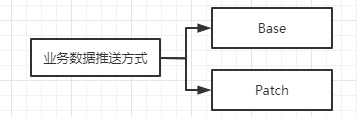
\includegraphics[height=3cm]{dataPush.png}
  \bicaption[推送方式]
    {推送方式示意图}
    {Schematic diagram of push mode}
 \label{fig:dataPush}
\end{figure}

实时系统的核心即后台向前端的数据推送模式。业务数据同时通过 Base 和 Patch 两种方式推送。

Patch 推送则是指对 Entity 与 View 的更新事件。Patch 推送产生的原因可能来自于用户,如某用户发送了一条消息,也可能来自于集群,如结束表决的定时任务到时间了。Patch 推送产生后,先更新 Entity,再更新 View,最后再进行推送。View 数据可通过有序的 Patch 推送计算出来。

Base 推送是指将某个 View 数据推送给前端。Base 推送产生的原因可能来自于用户请求,如初始化内容,也可能来自于服务端的定时推送,如管理人查看表决详情的服务端推送。

\subsubsection{数据更新}

Entity 数据的更新完全来源于 Patch 推送。

View 数据的更新来源于 Patch 推送以及定时的 Entity 重新聚合计算。Patch 推送可能会更新前端 View 中的 聚合数据。在该策略下,必须进行定时重新聚合计算。定时的重新聚合计算目的是进行 聚合数据 的修正。常规地,在定时重新聚合计算完成后,一个 Base 推送应该被发起。

同源数据并不会被主动更新,因为它是到 Entity 的引用,Entity 被更新则意味着同源数据被更新。

\subsection{数据流}
本节中 “连接” 指 WebSocket 协议的连接,而 “会话” 指用户对服务的请求上下文。
\subsubsection{用户建立会话数据流}
\begin{figure}[!htp]
  \centering
  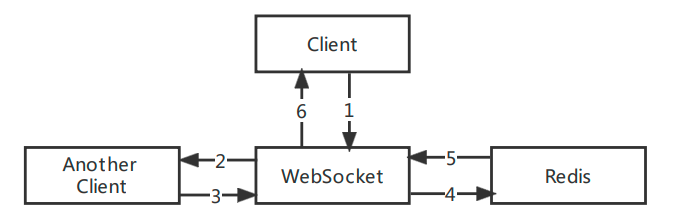
\includegraphics[width=12cm]{createDataflow.png}
  \bicaption[建立数据流]
    {用户建立会话数据流示意图}
    {Schematic diagram of user establishing session data flow}
 \label{fig:createDataflow}
\end{figure}
用户如果要与实例交互,必须先成功建立连接,然后建立会话。
会话是否建立及会话是否存在的判定均以是否建立会话数据,是否存在会话数据为准。
一个用户在同一时刻对一个实时服务只能有一个会话。

1. 客户端向 WebSocket 实例请求搭建连接,实例拿起该用户的会话并且建立锁,然后向 Redis 请求检查用户会话数据:

\quad{}a. 如果已经存在会话数据,并且通过会话数据判定连接未关闭,则转至第 2 步解决异地登陆。

\quad{}b. 如果已经存在会话数据,并且通过会话数据判定连接已关闭,则转至第 4 步覆盖会话;

\quad{}c. 如果检查发现不存在会话数据,则转至第 4 步建立会话;

2. 实例发现异地登录请求,通过 Redis 中的连接,通知占用会话的用户异地登陆的异常;

3. 实例通过清除 Redis 中的对应会话数据关闭与当前占用会话用户的连接,并且转至第 4 步覆盖会话;

4. 实例生成针对该用户的会话数据,与该用户建立连接,并将会话数据存入 Redis;

5. 实例保存会话数据至内存,同时保存当前连接。此时视为会话已经成功建立;

6. 实例放开该用户的会话建立锁,通知用户,会话建立成功,可以接受推送订阅和推送请求。
\subsubsection{用户请求数据流}
\begin{figure}[!htp]
  \centering
  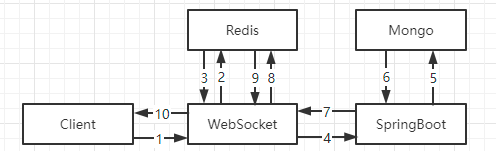
\includegraphics[width=12cm]{requestDateflow.png}
  \bicaption[请求数据流]
    {用户请求数据流示意图}
    {User request data flow diagram}
 \label{fig:requestDateflow}
\end{figure}
框架数据流整体过程如下:

1. 客户端向 WebSocket 实例发送请求:

\quad{}a. 如果 Redis 中已经缓存了相关数据,并且当前请求为读请求,则跳转至第 10 步;

\quad{}b. 如果 Redis 中已经缓存了相关数据,并且当前请求为写请求,则跳转至第 2 步;

\quad{}c. 如果 Redis 中没有相关数据的缓存数据,则直接跳转至第 4 步;

2. 根据写请求的具体要求,WebSocket 实例向 Redis 中写入/更新 Entity 和 View数据;

3. 根据写请求的具体要求,WebSocket 实例将相关数据写入实例内存中,转至第 10 步;

4. 若 Redis 没有缓存数据,则由 WebSocket 实例调用 SpringBoot 后端相关服务接口;

5. SpringBoot 后端向 Mongo 数据库请求获取相关 Entity 数据;

6. Mongo 数据将相关 Entity 数据返回至 SpringBoot 后端中;

7. SpringBoot 后端返回相关 Entity 数据,由 WebSocket 实例计算出相关 View 数据;

8. WebSocket 实例将相关 Entity 数据和 View 数据缓存到 Redis 中;

9. Redis 缓存 Entity 数据和 View 数据成功,WebSocket 也在实例内存中保存对应数据;

10. WebSocket 将请求结果返回给 Client。